%----------------------------------------------------------------------------
\chapter{Background}
%----------------------------------------------------------------------------

This chapter provides some theoretical background of the contributions presented in this thesis. First of all, the necessary basics of formal language and automaton theory are introduced, afterwards we discuss automaton learning algorithms.

\section{Basics of automaton theory}

First, we introduce the fundamentals of formal language theory, which are essential in order to understand automaton theory. Atomic elements of formal languages are alphabets, characters and words.

\begin{definition}[Alphabet]
	Let $\Sigma$ be a finite, non-empty set. $\Sigma$ is an Alphabet, its elements are symbols or characters.
\end{definition}

\begin{definition}[Word]
	If $\Sigma$ is an alphabet, then any finite sequence comprised of the symbols of $\Sigma$ are words (or Strings). $\Sigma^{n}$ represents the set of every n length word in $\Sigma$. The set of every word under an alphabet, formally $\bigcup\limits_{n>0}^{} \Sigma^{n}$ is denoted by $\Sigma^{*}$.
\end{definition}

\begin{definition}[Formal Language]
	An arbitrary set of words under an Alphabet $\Sigma$ is a Language. Formally: $L\subseteq\Sigma^{*}$.
\end{definition}

We will expand on formal languages more once we have a basic understanding of automatons. 

Informally, Automatons, or automata are mathematical constructs which are able to determine if a sequence of inputs should be accepted or rejected. A bit more precisely, automata consist of states and is always in one of them. Starting from an initial state, based on the inputs received, the automaton changes, "moves" between states. Essentially, for every one of the inputs, based on the current state the automaton is in, it determines whether to keep, or change its current state. In order to determine if an input sequence should be accepted or not, some states are special, accepting states. If after processing a sequence of inputs, the final state of the automaton is accepting, the input sequence is accepted. If not, the input is rejected.


One of the most simple automaton is the Deterministic Finite Automaton.

\begin{definition}[Deterministic Finite Automaton]
	A Deterministic Finite Automaton is a Tuple of $ DFA=(S,s_{0},\Sigma,\delta,F) $, where: 
	\begin{itemize}
		\item S is a finite, non-epty set containing the states of the automaton,
		\item $s_{0} \in S$ is the initial state,
		\item $\Sigma$ is a finite Alphabet,
		\item $\delta: S\times \Sigma \to S$ is a transition function,
		\item $F\subseteq S$ is a set of the accepting states of the automaton. 
	\end{itemize}
\end{definition}


An example of a DFA (Deterministic Finite Automaton) from\cite{Steffen2011} can be seen in Fig. \ref{fig:dfaexample}. This example has four states, $S = \{q_0, q_1, q_2, q_3\}$ (hence $|S| = 4$). The initial state is marked by the start arrow, so $s_0 = q_0$. The alphabet can be inferred as $\Sigma = \{a, b\}$ because of the deterministic in Deterministic Finite automaton, meaning every state must deterministically know what input causes what action. This means, that every state must have every member of the alphabet listed in its transitions. Transitions being the from\_state $\xrightarrow[]{\text{input}}$ to\_state given by the transition function e.g. $\delta(q_0, a) = q_1$. The whole of the transition function in a table form can be seen in Table \ref{tab:dfaexampledelta}. Finally, the accepting states, or in this case, accepting state of the automaton is $F = \{q_3\}$.

When talking about automata, it is important to discuss runs. A run of an automaton is to test for a certain input (word), if it is accepted or rejected. An example run of Fig. \ref{fig:dfaexample} with an input of $\{a, a, a\}$ would (following the transition function) end in state $q_3$ meaning the input is accepted. A rejected input could be $\{a, b, b\}$, which would stop at state $q_1$, a non-accepting state. On deeper examination, one can see, that this automaton only accepts runs with inputs containing $4i+3 a$.

\begin{figure}[H]
	\centering
	\begin{tikzpicture}[shorten >=1pt,node distance=3cm,on grid,auto] 
	\node[state,initial] (q_0)   {$q_0$}; 
	\node[state] (q_1) [right=of q_0] {$q_1$}; 
	\node[state] (q_2) [below=of q_0] {$q_2$}; 
	\node[state,accepting](q_3) [right=of q_2] {$q_3$};
	\path[->] 
	(q_0) edge  node {a} (q_1)
	edge [loop below] node {b} ()
	(q_1) edge  node  {a} (q_2)
	edge [loop below] node {b} ()
	(q_2) edge  node [swap] {a} (q_3) 
	edge [loop above] node {b} ()
	(q_3) edge  node [swap] {a} (q_0)
	 edge [loop above] node {b} () ;
	\end{tikzpicture}
	\caption{A simple DFA}
	\label{fig:dfaexample}
\end{figure}

\begin{table}[H]
\centering
\begin{tabular}{|c|cccc|}
	\hline
	$\delta$ & $q_0$ & $q_1$ & $q_2$ & $q_3$\\ \cline{1-5}
	a & $q_1$ & $q_2$ & $q_3$ & $q_0$ \\	
	b & $q_0$ & $q_1$ & $q_2$ & $q_3$ \\	\hline
\end{tabular}
\caption{The transition function of the automaton seen in Fig. \ref{fig:dfaexample}}
\label{tab:dfaexampledelta}
\end{table}

DFAs are great to model system behavior based on inputs, but in order to work with reactive systems, we also need to handle outputs. Mealy machines are automata designed to do just this, but the accepting of an input sequence is a bit more complicated.


\begin{definition}[Mealy machine]
	A Mealy machine or Mealy automaton is a Tuple of $ M=(S,s_{0},\Sigma,\Omega,\delta,\lambda) $, where:
	\begin{itemize}
		\item S S is a finite, non-epty set containing the states of the automaton,
		\item $s_{0} \in S$ is the initial state,
		\item $\Sigma$ is the input alphabet of the automaton,
		\item $\Omega$ is the output alphabet of the automaton,
		\item $\delta: Q\times \Sigma \to Q$ is the transition function and
		\item $\lambda: Q\times \Sigma \to \Omega$ is the output function. 
	\end{itemize}
\end{definition}

\noindent Mealy machines can be regarded as deterministic finite automata over the union of the input alphabet and an output alphabet with just one rejection state, which is a sink, or more elegantly, with a partially defined transition relation. An example can be seen here:

\begin{figure}[H]
	\centering
	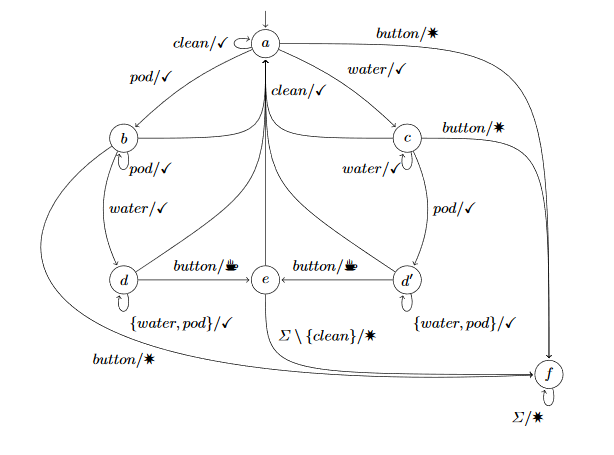
\includegraphics[width=0.7\linewidth]{content/coffeemealy}
	\caption{Mealy machine representing the functionality of a coffee machine.\cite{Steffen2011}}
	\label{fig:coffeemealy}
\end{figure}


\begin{definition}[Canonical automaton]
	An automaton accepting the language L is canonical iff it is minimal, and contains every other automaton that accepts L.
\end{definition}

\section{Automaton learning}



\paragraph{Automaton learning}  is the process of modeling a system without having specific knowledge of the internal workings of it. To accomplish this, we need to infer a model by observing its external behavior. This learned model is, as the name suggests, an automaton. 
\\Formally: Active  automata  learning is  concerned  with  the  problem  of  inferring  an automaton model for an unknown formal language $L$ over some alphabet $\Sigma$\cite{Howar2018}.
\\\\In order to monitor a system, we need a way of access to its behavioral information, for which there are two approaches, these separate the two types of automaton learning as well.

\paragraph{Passive automaton learning} is the case when the gathering of information is not part of the learning process, but rather a prerequisite to it. The learning is done on a pre-gathered positive an/or negative example set of the systems behavior. In passive automaton learning, the success of the process is not only determined by the efficiency of the algorithm, but the methodology and time used to gather the data.

\paragraph{Active automaton learning} is when the behavioral infromation is gathered by the learning algorithm in an "active" way via queries. For this there is a need to distinguish a learner and a teacher component, of which the second can answer basic questions about the system in real-time. 


\paragraph{MAT modell} Active automaton learning follows the MAT, or the Minimally Adequate Teacher model proposed by Dana Angluin\cite{ANGLUIN198787}. It separates the algorithm to a learner and a teacher, where the teacher can only answer the minimally adequate questions needed to learn the system. These two questions, or more precisely, queries are:


\paragraph{Membership query} Given a $w\in\Sigma^{*}$ word, it return the $o\in \Omega$ output corresponding to it, treating the word as a string of inputs.

\paragraph{Equivalence query} Given an $M$ hypothesis automaton, it tries to provide a counterexample $o\in\Omega$ and a $w\in\Sigma$ corresponding to it, where given the input $w$ to $M$ and the system, the output given by them differs. $o$ is the differring output given by the system. If no such counterexample can be found, M hypothesis is considered behaviorally identical to the monitored system.

\noindent The learner uses membership queries to build a hypothesis automaton, then refines these by equivalence queries. Once counterexamples can not be found this way, the learning terminates, the output is the current hypothesis.

